\section{Sprint 3 – Credit Management}

In this section, we first detail the Sprint 3 backlog, then present the design and implementation of features through screenshots and diagrams.

\subsection{Sprint 3 Backlog}

\begin{table}[!htbp]
  \centering
  \small
  \caption{Sprint 3 Backlog} 
  \label{tab:backlog_sprint3}
  \renewcommand{\arraystretch}{1.2}
  \begin{tabular}{|p{1cm}|p{4cm}|p{7cm}|p{2cm}|}
    \hline
    \textbf{ID} & \textbf{User Story}               & \textbf{Description}                                                                                             & \textbf{Priority} \\ \hline
    US7         & Purchase bulk credit & As a corporate user, I want to purchase bulk credit for my organization to enable payment transactions for end users. & High            \\ \hline
    US8         & Distribute credit across end users       & As a corporate user, I want to distribute purchased credit across my end users to enable their payment capabilities. & Critical         \\ \hline
    US9         & Monitor end users transactions       & As a corporate user, I want to monitor all end user transactions to track credit usage and maintain oversight. & Medium          \\ \hline
  \end{tabular}
\end{table}

\vspace{4cm}

\subsection{Use Case Diagram}
Figure~\ref{fig:uc_sprint3} presents the three major use cases developed during Sprint 3: purchasing bulk credit, distributing credit across end users, and monitoring end user transactions. It illustrates their respective interactions with the \textit{Corporate} actor and the authentication system.

\begin{figure}[htbp]
  \centering
  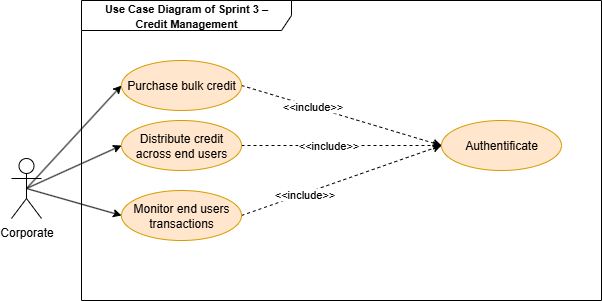
\includegraphics[width=0.9\textwidth]{images/usecase_sprint3.png}
  \caption{Use Case Diagram – Sprint 3}
  \label{fig:uc_sprint3}
\end{figure}

\subsection{Use Case Descriptions – Sprint 3}
In this section, we detail each use case identified for Sprint 3.

\vspace{4cm}

\subsubsection{Use Case "Purchase bulk credit"}
\begin{longtable}{|p{0.2\textwidth}|p{0.75\textwidth}|}

  \caption{Description of use case "Purchase bulk credit"}
  \label{tab:uc_purchase_bulk_credit} \\
  \hline
  \textbf{Title} & Purchase bulk credit \\ \hline
  \textbf{Actors} & Corporate \\ \hline
  \textbf{Description} & The corporate user purchases bulk credit for their organization through email verification and admin approval process. \\ \hline
  \textbf{Preconditions} & 
    \begin{itemize}[nosep,leftmargin=*]
      \item The corporate user is authenticated with valid credentials.
      \item The corporate user has sufficient funds or valid payment method.
      \item Admin server is available for transaction processing.
    \end{itemize} \\ \hline
  \textbf{Postconditions} & 
    \begin{itemize}[nosep,leftmargin=*]
      \item Bulk credit is purchased and added to corporate balance.
      \item Transaction record is created with purchase details.
      \item Corporate user receives confirmation of successful purchase.
    \end{itemize} \\ \hline
  \textbf{Main Scenario} &
    \begin{enumerate}[nosep,leftmargin=*]
      \item Corporate user selects "Purchase Bulk Credit" option.
      \item System displays credit purchase form with amount selection.
      \item Corporate user enters desired credit amount and confirms.
      \item System sends email verification to corporate user.
      \item Corporate user confirms via email verification link.
      \item System forwards transaction to admin server for processing.
      \item Admin accepts the payment and provides credit to corporate.
      \item System updates corporate total balance with purchased credit.
      \item Corporate user receives success confirmation message.
    \end{enumerate} \\ \hline
  \textbf{Alternative Scenarios} &
    \begin{enumerate}[nosep,leftmargin=*]
      \item If corporate user cancels purchase, return to main dashboard.
      \item If email verification expires, resend verification email.
    \end{enumerate} \\ \hline
  \textbf{Exception Scenarios} &
    \begin{enumerate}[nosep,leftmargin=*]
      \item If admin refuses payment, display "Payment rejected" with rejection email.
      \item If transaction processing fails, show "Transaction failed, please retry".
      \item If network timeout occurs, display "Connection error, please retry".
    \end{enumerate} \\ \hline

\end{longtable}

\vspace{1cm}

\subsubsection{Use Case "Distribute credit across end users"}
\begin{longtable}{|p{0.2\textwidth}|p{0.75\textwidth}|}
  \caption{Description of use case "Distribute credit across end users"}
  \label{tab:uc_distribute_credit} \\
  \hline
  \textbf{Title} & Distribute credit across end users \\ \hline
  \textbf{Actors} & Corporate \\ \hline
  \textbf{Description} & Corporate user distributes purchased credit to end users within their organization, with balance validation and transaction processing. \\ \hline
  \textbf{Preconditions} & 
    \begin{itemize}[nosep,leftmargin=*]
      \item Corporate user is authenticated and has sufficient credit balance.
      \item End users are registered within the corporate organization.
      \item Transaction controller is operational for processing.
    \end{itemize} \\ \hline
  \textbf{Postconditions} & 
    \begin{itemize}[nosep,leftmargin=*]
      \item Credit is successfully distributed to selected end users.
      \item Corporate balance is reduced by distributed amount.
      \item End users receive credit allocation notifications.
    \end{itemize} \\ \hline
  \textbf{Main Scenario} &
    \begin{enumerate}[nosep,leftmargin=*]
      \item Corporate user selects "Distribute Credit" option.
      \item System displays list of end users and distribution form.
      \item Corporate user selects end users and specifies credit amounts.
      \item System validates corporate balance sufficiency.
      \item Transaction controller processes credit distribution.
      \item System updates corporate balance and end user balances.
      \item Corporate user receives success confirmation message.
    \end{enumerate} \\ \hline
  \textbf{Alternative Scenarios} &
    \begin{enumerate}[nosep,leftmargin=*]
      \item If corporate user modifies distribution, recalculate totals.
      \item If partial distribution succeeds, show successful and failed allocations.
    \end{enumerate} \\ \hline
  \textbf{Exception Scenarios} &
    \begin{enumerate}[nosep,leftmargin=*]
      \item If insufficient balance, display "Not enough balance, credit distribution cancelled".
      \item If transaction processing fails, show "Distribution failed, please retry".
      \item If end user account is inactive, skip and notify corporate user.
    \end{enumerate} \\ \hline

\end{longtable}

\vspace{3cm}

\subsubsection{Use Case "Monitor end users transactions"}
\begin{longtable}{|p{0.2\textwidth}|p{0.75\textwidth}|}
  \caption{Description of use case "Monitor end users transactions"}
  \label{tab:uc_monitor_transactions} \\
  \hline
  \textbf{Title} & Monitor end users transactions \\ \hline
  \textbf{Actors} & Corporate \\ \hline
  \textbf{Description} & Corporate user monitors all end user transactions within their organization to track credit usage and maintain oversight. \\ \hline
  \textbf{Preconditions} & 
    \begin{itemize}[nosep,leftmargin=*]
      \item Corporate user is authenticated with monitoring permissions.
      \item Transaction data is available in the system database.
      \item End users have performed transactions to monitor.
    \end{itemize} \\ \hline
  \textbf{Postconditions} & 
    \begin{itemize}[nosep,leftmargin=*]
      \item Transaction monitoring data is retrieved and displayed.
      \item Corporate user can filter and analyze transaction patterns.
      \item Monitoring activity is logged for audit purposes.
    \end{itemize} \\ \hline
 \textbf{Main Scenario} &
    \begin{enumerate}[nosep,leftmargin=*]
      \item Corporate user opens "Monitor Transactions" dashboard.
      \item System retrieves all end user transaction data.
      \item Transaction data is processed and formatted for display.
      \item Interface displays transaction history with filtering options.
      \item Corporate user can view detailed transaction information.
      \item System provides analytics and usage summaries.
    \end{enumerate} \\ \hline
  \textbf{Alternative Scenarios} &
    \begin{enumerate}[nosep,leftmargin=*]
      \item If no transactions exist, display "No transactions found".
      \item If date filter returns no results, show "No results for selected period".
    \end{enumerate} \\ \hline
  \textbf{Exception Scenarios} &
    \begin{enumerate}[nosep,leftmargin=*]
      \item If monitoring service fails, display "Failed to load transaction data".
      \item If data access is restricted, show "Insufficient permissions".
    \end{enumerate} \\ \hline

\end{longtable}

\vspace{5cm}

\subsection{Sequence Diagrams}

\subsubsection{Sequence Diagram - Purchase Bulk Credit}
This diagram (see figure \ref{fig:seq_purchase_bulk_credit}) models the bulk credit purchase process with email verification and admin approval:
\begin{itemize}[nosep,leftmargin=*]
  \item Corporate user initiates bulk credit purchase request.
  \item System sends email verification and waits for confirmation.
  \item Upon email confirmation, transaction is forwarded to admin server.
  \item Admin processes payment and either accepts or refuses the transaction.
  \item System updates corporate balance and provides confirmation.
\end{itemize}

\begin{figure}[H] 
  \centering
  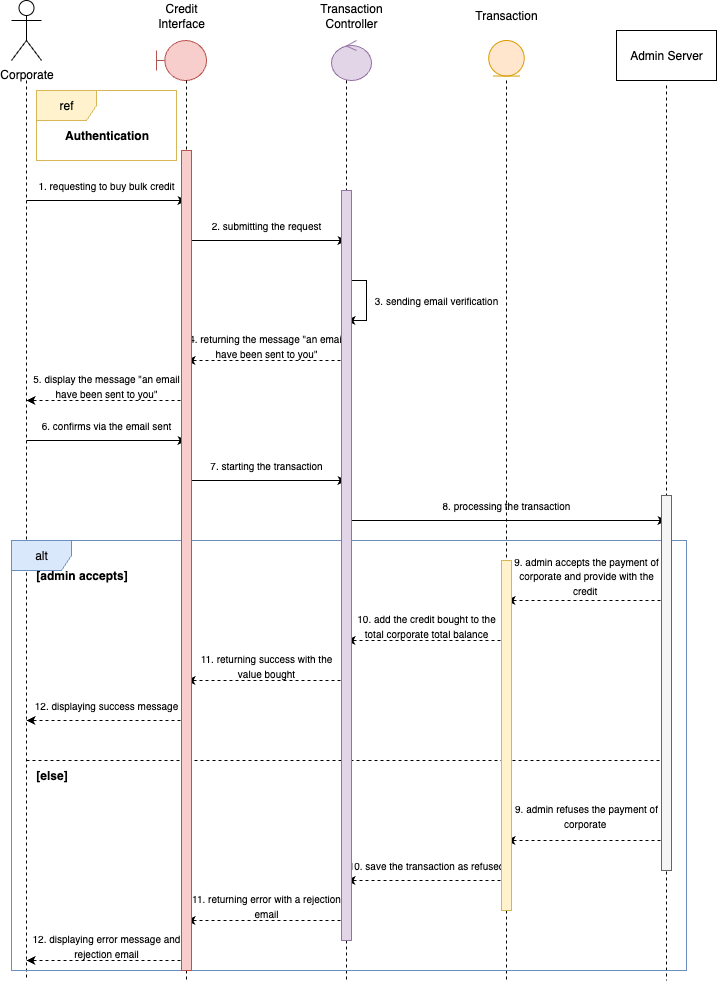
\includegraphics[width=\textwidth,keepaspectratio]{images/seq_purchase_bulk_credit.png}
  \caption{Sequence Diagram "Purchase Bulk Credit"}
  \label{fig:seq_purchase_bulk_credit}
\end{figure}

\subsubsection{Sequence Diagram - Distribute Credit Across End Users}
This diagram (see figure \ref{fig:seq_distribute_credit}) shows the credit distribution process with balance validation:
\begin{itemize}[nosep,leftmargin=*]
  \item Corporate user requests to distribute credits to end users.
  \item System validates corporate balance sufficiency.
  \item Transaction controller processes the credit distribution.
  \item System updates balances and provides success confirmation.
\end{itemize}

\begin{figure}[H] 
  \centering
  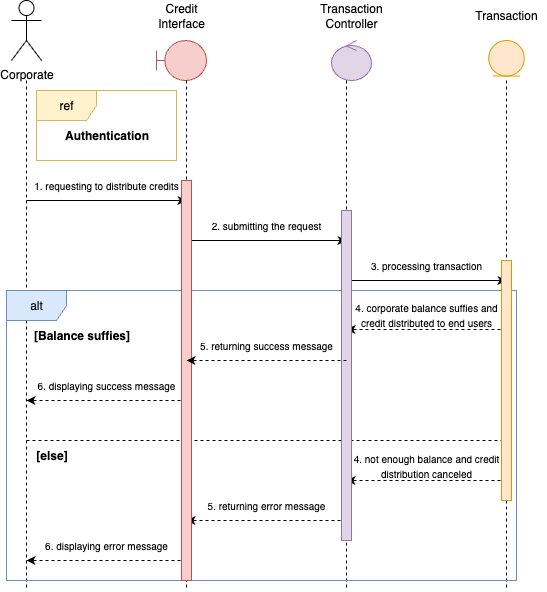
\includegraphics[width=\textwidth,keepaspectratio]{images/seq_distribute_credit_across_end_users.png}
  \caption{Sequence Diagram "Distribute Credit Across End Users"}
  \label{fig:seq_distribute_credit}
\end{figure}

\subsection{Class Diagram (Sprint 3)}

The enriched class diagram for Sprint 3 adds new business entities for credit management:

\begin{itemize}[nosep,leftmargin=*]
  \item \textbf{CorporateAccount}: manages corporate user accounts and credit balances;
    \begin{itemize}[nosep,leftmargin=*,label=•]
      \item corporate account identifier (\texttt{id});
      \item organization name (\texttt{organizationName});
      \item total credit balance (\texttt{creditBalance});
      \item account creation date (\texttt{createdAt});
      \item account status (\texttt{status}).
    \end{itemize}

  \item \textbf{CreditTransaction}: stores credit purchase and distribution records;
    \begin{itemize}[nosep,leftmargin=*,label=•]
      \item transaction identifier (\texttt{id});
      \item corporate account reference (\texttt{corporateId});
      \item transaction type (\texttt{type}: \texttt{PURCHASE}, \texttt{DISTRIBUTION});
      \item credit amount (\texttt{amount});
      \item transaction timestamp (\texttt{timestamp});
      \item transaction status (\texttt{status}: \texttt{PENDING}, \texttt{APPROVED}, \texttt{REJECTED}).
    \end{itemize}
\end{itemize}

% \begin{figure}[H]
% \centering  
% \includegraphics[width=1\textwidth]{images/class_diagram_sprint3.png}
% \caption{Class Diagram – Sprint 3}
% \label{fig:class_sprint3}
% \end{figure}

\subsection{Realization (Sprint 3)}

In this section, we present the main interfaces developed during Sprint 3, dedicated to credit management functionality. This work involved implementing bulk credit purchasing, credit distribution systems, and transaction monitoring capabilities. Each interface is illustrated with screenshots and accompanied by descriptions of functionality and user journey.

\subsubsection{Bulk credit purchase interface}

The bulk credit purchase interface guides corporate users through the credit purchasing process with email verification and admin approval.

\noindent\textbf{Credit Purchase Form:}

Figure \ref{fig:credit_purchase_form} illustrates the credit purchase form, the initial step of the bulk credit acquisition process.

% \begin{figure}[H]
%   \centering
%   \includegraphics[width=0.8\textwidth,keepaspectratio]{images/credit_purchase_form.png}
%   \caption{Credit purchase form with amount selection}
%   \label{fig:credit_purchase_form}
% \end{figure}

— \textbf{States presented:}
\begin{itemize}[nosep,leftmargin=*,label=•]
  \item \textbf{Amount selection}  
    Corporate user selects desired credit amount with pricing display.
  \item \textbf{Payment method}  
    Selection of payment method and billing information.
  \item \textbf{Email verification}  
    System sends verification email for transaction security.
\end{itemize}

— \textbf{Credit purchase flow:}
\begin{itemize}[nosep,leftmargin=*,label=•]
  \item Corporate user is authenticated and accesses purchase form.
  \item User selects credit amount and confirms purchase details.
  \item System sends email verification for security confirmation.
  \item Upon email verification, transaction is sent to admin for approval.
  \item Admin processes payment and credits are added to corporate balance.
\end{itemize}

\subsubsection{Credit distribution dashboard}

The credit distribution dashboard enables corporate users to allocate purchased credit across their end users (see Figure \ref{fig:credit_distribution}).

% \begin{figure}[H]
%   \centering
%   \includegraphics[width=\textwidth,keepaspectratio]{images/credit_distribution_dashboard.png}
%   \caption{Credit Distribution Dashboard}
%   \label{fig:credit_distribution}
% \end{figure}

— \textbf{States presented:}
\begin{itemize}[nosep,leftmargin=*,label=•]
  \item \textbf{End user list}  
    Display of all end users within the corporate organization.
  \item \textbf{Credit allocation}  
    Input fields for specifying credit amounts per user.
  \item \textbf{Balance validation}  
    Real-time validation of sufficient corporate balance.
  \item \textbf{Distribution confirmation}  
    Summary and confirmation of credit distribution.
\end{itemize}

— \textbf{Credit distribution flow:}
\begin{itemize}[nosep,leftmargin=*,label=•]
  \item Corporate user accesses distribution dashboard.
  \item System displays list of end users and current balances.
  \item User specifies credit amounts for selected end users.
  \item System validates sufficient corporate balance for distribution.
  \item Upon confirmation, credits are distributed and balances updated.
\end{itemize}
